\chapter{MANTA/FLIP} 
\label{sec:ships}
\lstset{style=6502Style}

Perhaps one of the lovelist accomplishments in \textit{Uridium} is the animation the game
performs when the player's manta changes horizontal direction. There is a suprising amount
of depth to the way this maneouvre is rendered and it contains a number of subtle details
that evidence the care and attention that was paid to its implementation. Together with
the silky scrolling I believe the endeavour for detailed realism in this animation
is responsible for the immersion this game creates, even for the modern player. 

The first remarkable thing about the manouevre is the sheer number of sprites that are
devoted to it. In the impressionistic rendering below you get a sense of how dense
the animation is, how many individual frames have been devoted to its creation.

\begin{figure}[H]
    \centering
    \begin{adjustbox}{width=13cm,center}
      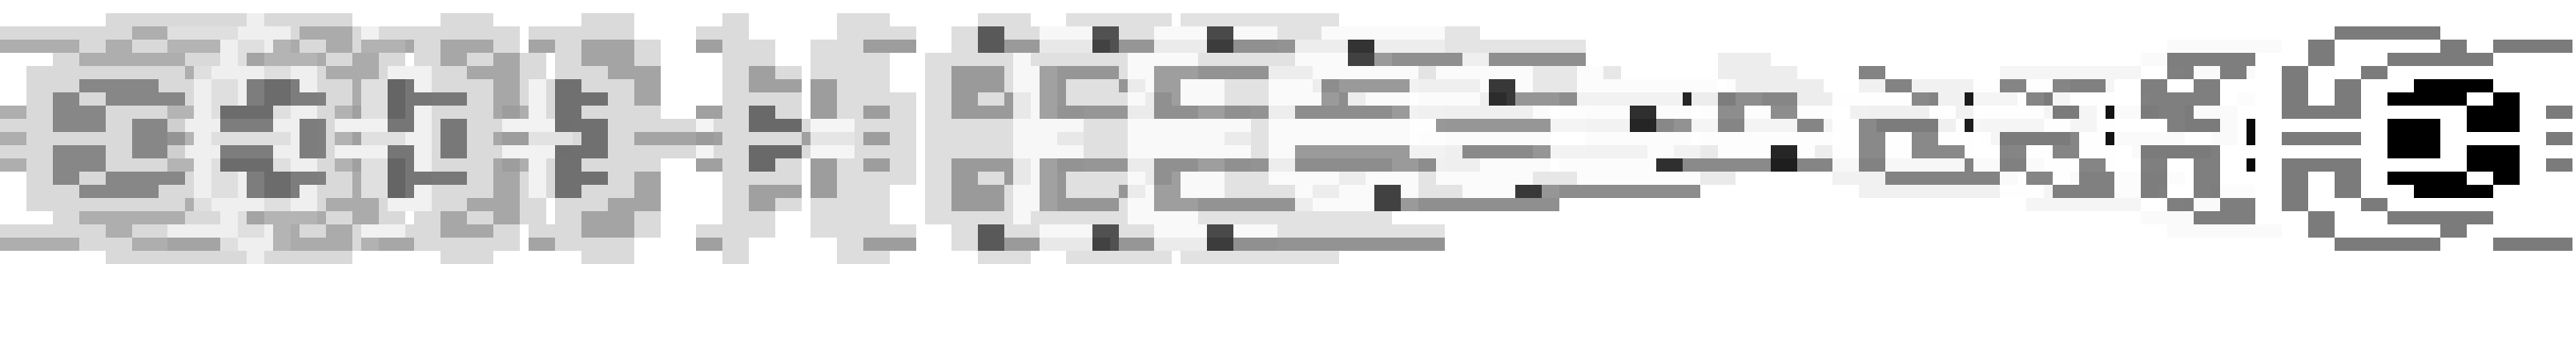
\includegraphics[width=15cm]{src/manta_flip/manta_flip.png}%
    \end{adjustbox}
\end{figure}
\vspace{-0.5cm}

If we unpick this impressionistic rendering and show each sprite in isolation we get
a better sense of just how many are involved, 16 in total.
\begin{figure}[H]
    \hspace{0.2cm}
    \begin{adjustbox}{width=13.5cm,center}
      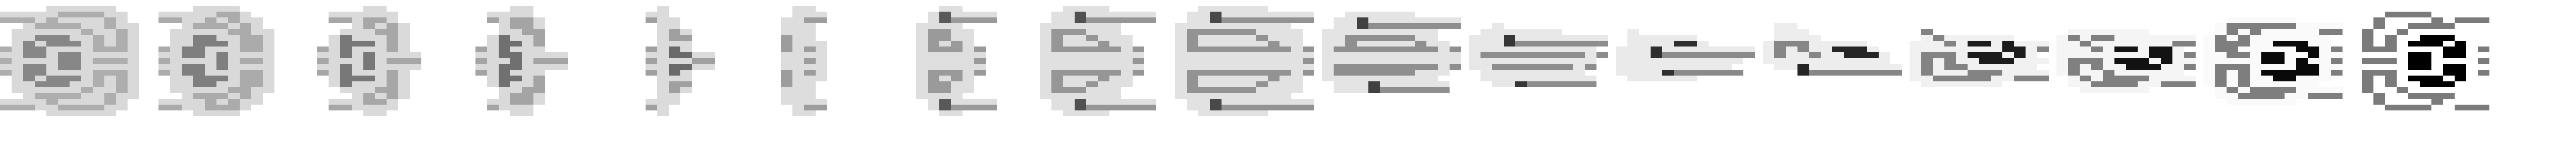
\includegraphics[width=15cm]{src/manta_flip/manta_flip_wide.png}%
    \end{adjustbox}
\end{figure}
\vspace{-0.5cm}

As we look closer we can see the manouevre is broken up into two parts: a flip, and a roll.
It is no coincidence that these two elements to the manouvre are symmetrical in length, this
symmetry is part of what underlines its visual appeal. The flip occurs over eight individual
frames.
\begin{figure}[H]
    \centering
    \begin{adjustbox}{width=13cm,center}
      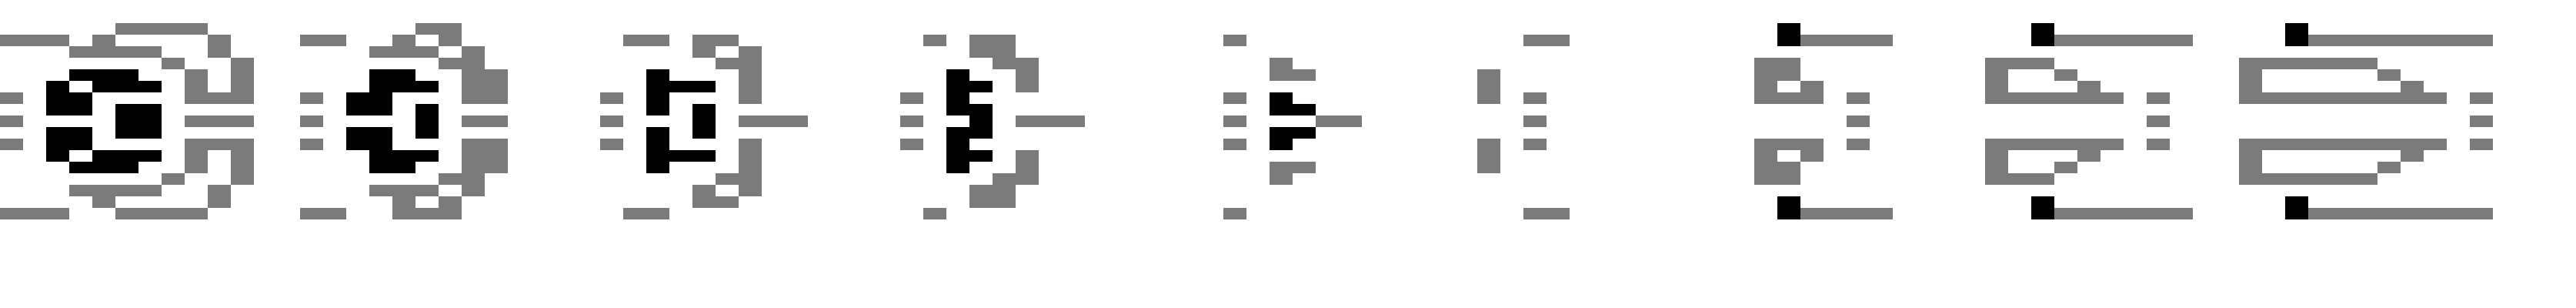
\includegraphics[width=15cm]{src/manta_flip/manta_flip_1.png}%
    \end{adjustbox}
\end{figure}
\vspace{-0.5cm}

The roll is the same, the manta rotates a full 180 degrees, completing the turn.
\begin{figure}[H]
    \centering
    \begin{adjustbox}{width=13cm,center}
      
\includegraphics[width=15cm]{src/manta_flip/manta_flip_2.png}%
    \end{adjustbox}
\end{figure}
\vspace{-0.5cm}

Notice how we could break each of these halves of the manouevre equally again. Each reaches
its halfway point in the very middle. 

Of course, as we must expect by now, a sequence like this must be governed by a data structure.
This is provided by \icode{mantaFlipFromLeftToRight} which we give below. The main body of this
structure is, as we would expect, the sequence of sprite values that make up the frames of the
animation.

\begin{lstlisting}[basicstyle=\footnotesize\ttfamily]
mantaFlipFromLeftToRight
  .BYTE 16                                  ; No. of Frames in Animation
  .BYTE $41,$40,$4F,$4E,$4D,$4C,$4B,$4A     ; Sprites for the roll..
  .BYTE $49,$67,$68,$69,$6A,$6B,$6C,$6D,$59 ; .. and the flip.
  .BYTE $28                                 ; Whether to adjust shadow.
\end{lstlisting}

If we compare the data structure used to define the animation with the order of the frames
below we can see that they are utilized in reverse order. We start at the end with sprite \icode{\$59}
and end on sprite \icode{\$41}.

\begin{figure}[H]
    \centering
    \begin{adjustbox}{width=13cm,center}
      
\includegraphics[width=15cm]{src/manta_flip/6_mantaFlipFromLeftToRight_0.png}%
    \end{adjustbox}
    \vspace{0.2cm}
    \begin{adjustbox}{width=13cm,center}
      
\includegraphics[width=15cm]{src/manta_flip/6_mantaFlipFromLeftToRight_8.png}%
    \end{adjustbox}
\end{figure}
\vspace{-0.5cm}

But there is more to the data structure than just this. Our comment on the last byte mentions something
do with a shadow adjustment. To see what this might be we need to take a look at how the animation is
rendered over the surface of a dreadnought.

\begin{figure}[H]
    \centering
    \begin{adjustbox}{width=13cm,center}
      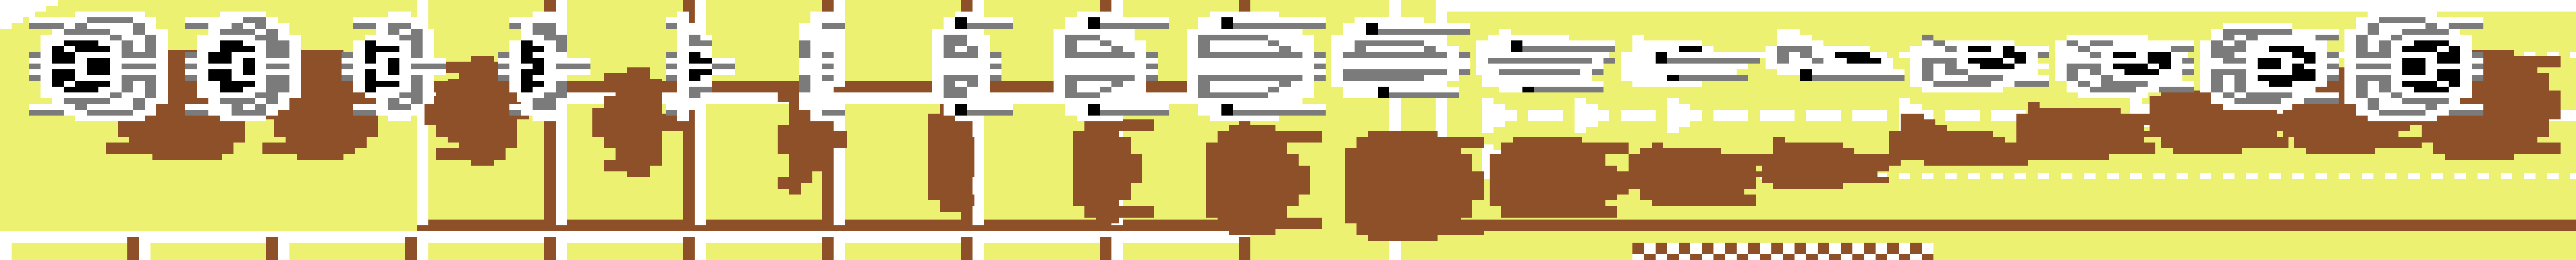
\includegraphics[width=15cm]{src/manta_flip/flip_diagram.png}%
    \end{adjustbox}
\end{figure}
\vspace{-0.5cm}

Perhaps it is not immediately obvious? Pay attention to the behaviour of the shadows below the manta.
It might be easier to notice the effect if we zoom into the \icode{flip}.

\begin{figure}[H]
    \centering
    \begin{adjustbox}{width=13cm,center}
      
\includegraphics[width=15cm]{src/manta_flip/flip_diagram_1.png}%
    \end{adjustbox}
\end{figure}
\vspace{-0.5cm}

If it is still not obvious, that might a testament to the realism of the effect. You are seeing what
you expect to see, so nothing stands out. The hidden hand of extreme attention to detail has concealed
its workings from you. Let's see if you can see something wrong if we remove the effect:

\begin{figure}[H]
    \centering
    \begin{adjustbox}{width=13cm,center}
      
\includegraphics[width=15cm]{src/manta_flip/flip_diagram_1_no_offset.png}%
    \end{adjustbox}
\end{figure}
\vspace{-0.5cm}

Hopefully it is evident now: as the player's ship flips back the shadow on the surface of the dreadnought
moves away from the manta. This is not happening by accident, but because it had to be implemented specifically
to create the impression that the manta is lifting up from the surface as it turns back in on itself. 

As the manta rolls, it returns towards the surface, eventually resuming its original altitude. As it does so,
its shadow gets closer.

\begin{figure}[H]
    \centering
    \begin{adjustbox}{width=13cm,center}
      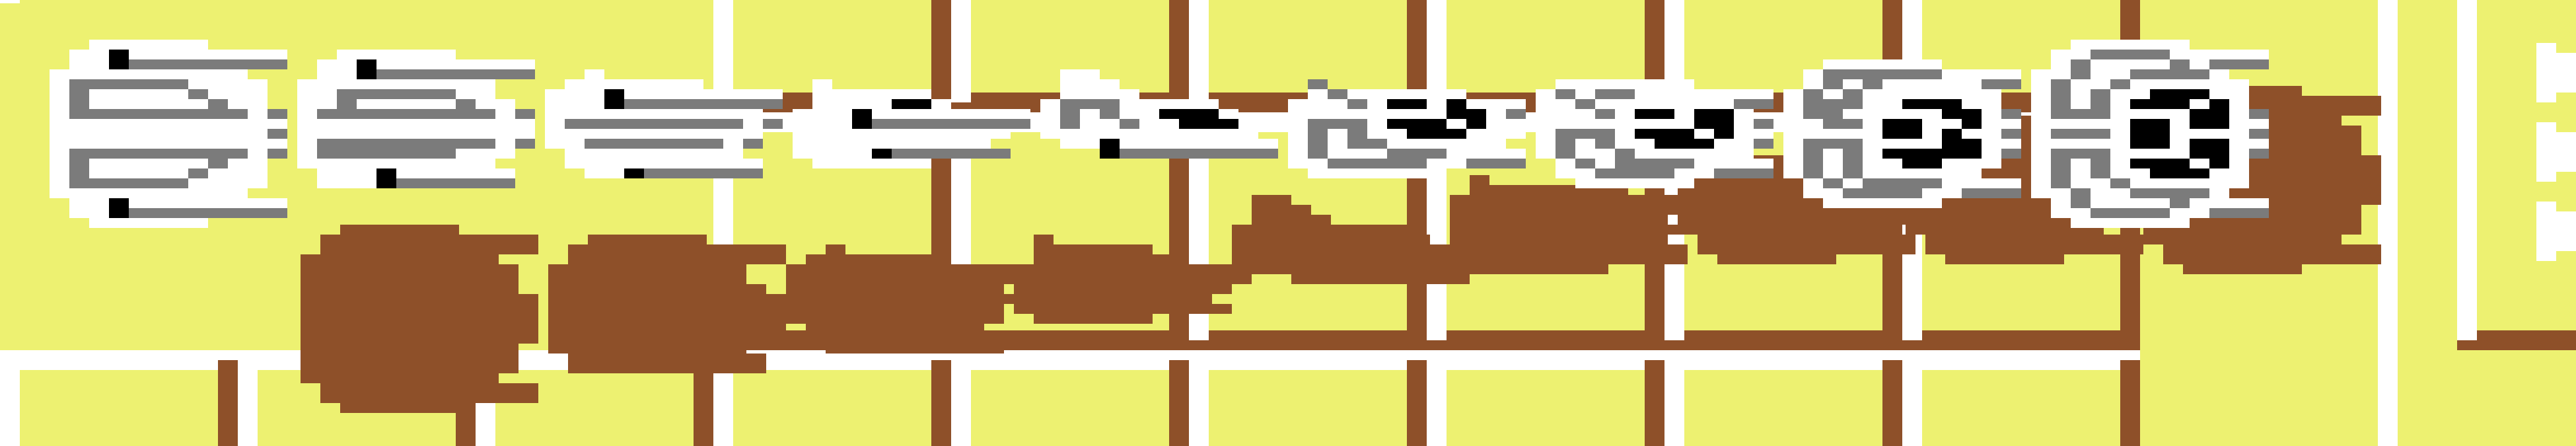
\includegraphics[width=15cm]{src/manta_flip/flip_diagram_2.png}%
    \end{adjustbox}
\end{figure}
\vspace{-0.5cm}

Underlying this effect is an array of offsets, each one paired with a frame in the animation. And like the
animation in \icode{mantaFlipFromLeftToRight}, this array is designed to be read from the end. This means
we can use the same index we use to read in sprite frames from \icode{mantaFlipFromLeftToRight} to read in the 
the appropriate offset to add to the position of the sprite's shadow.

The array is given below. Interesting to note is the way the movement of the shadow is designed to speed up and
then slow down before arriving at its peak altitude, and likewise when descending back to the surface.

\begin{lstlisting}
mantaShadowOffsets   
  .CHAR  0,-1,-2,-3,-3,-2,-2, -1 ; Shadow moves towards the manta (Roll).
  .CHAR  0, 1, 2, 3, 3, 2, 2,  1 ; Shadow moves away from the manta (Flip).
\end{lstlisting}

This naturalistic movement is emblematic of the kind of deep consideration this manoeuvre has been given. Not only
has serious thought been given to conveying the vertical movement of the player's ship, but the game has found a way
of expressing the acceleration and deceleration that would be inherent to a flip and roll of this sort.

On the opposite page we can seehow all of this, the \icode{mantaFlipFromLeftToRight} animation data structure, 
plus the \icode{mantaShadowOffsets} array, come together in a short routine that combines them both to fetch a
new frame of the animation and update the position and appearance of the  manta and shadow sprites as appropriate.

Note how there are two things determining whether we should draw a new frame of the animation. The first is
\icode{mantaState} which, if an animation is active, will have its top bit set (e.g. \icode{\$80}, making it 
a negative value). The second is the \icode{frameRate}: since this routine may be visited dozens of times a
second it will only ever need to do anything new once the current frame of the animation has been displayed
for a long enough period.

\clearpage
\begin{lstlisting}[basicstyle=\scriptsize\ttfamily]
;-----------------------------------------------------------------------------
; Draw a frame from a manouevre animation (in our example, mantaFlipFromLeftToRight)..
; This routine called by the main game loop dozens of times a second!
;-----------------------------------------------------------------------------
DrawTheAnimation   
  LDA mantaState                       ; Check if we should draw a new frame.
  BMI GetNextFrameOfAnimation          ; If so, then get the next frame..
  JMP DrawMantaAnimationFrame          ; Otherwise just redraw the current one.

GetNextFrameOfAnimation
  ; Check our frame rate before displaying a new one.
  LDA frameRate                        ; Check if we should display new frame. 
  AND #$01                             ; If it's an odd number, get a new frame.
  BNE DrawMantaAnimationFrame          ; Otherwise draw the current one again.

  ; Get the new sprite. mantaAnimationLoPtr is a pointer into the
  ; mantaFlipFromLeftToRight animation data structure (in this example).
  LDY currentFrame                     ; Get the current frame index.
  LDA (mantaAnimationLoPtr),Y          ; Get next sprite from the data structure.
  STA newSpriteValue                   ; Store it as the new sprite frame.

  ; Get the shadow offset for this frame of the animation.
  ; We will only do this if the appropriate byte is non-zero in the animation's
  ; data structure.
  LDA shadowDepthDuringMantaAnimation  ; Check whether to display a shadow.
  BEQ DecrementFrameIndex              ; If not, skip adding the shadow offset.
  LDA mantaShadowOffsets,Y             ; Get shadow offset for new frame.
  ADC mantaShadowOffset                ; Add the current offset to it.
  STA mantaShadowOffset                ; Store as the new shadow offset.
DecrementFrameIndex
  DEC currentFrame                     ; Decrement frame index for next time around.

  ; Draw the animation frame.
DrawMantaAnimationFrame   
  LDA #$06                             ; Get sprite index for the manta.
  STA spriteIndex                      ; Store it in spriteIndex.
  JSR GetCurrentSprite                 ; Load current sprite info for the manta.
  LDA newSpriteValue                   ; Get our new frame and..
  STA currentSpriteValue               ; .. update the manta sprite with it.
  ADC #$30                             ; Add $30 to point A to the shadow sprite.
  STA mantaShadowSpriteValue           ; Store the new frame in it too.
  LDA mantaCurrentYPos                 ; Get manta's current Y position.
  STA currentSpriteYPos                ; Store it as the manta sprite's position.
  JSR DisplayCurrentSprite             ; Display the manta sprite with the new values.

  ; Draw the Manta's shadow.
  INC spriteIndex                      ; Move sprite index to point to the shadow.
  JSR GetCurrentSprite                 ; Load current sprite info for the shadow.
  LDA mantaShadowSpriteValue           ; Get the new sprite for the shadow.
  STA currentSpriteValue               ; .. and update the shadow sprite with it.

  ; Calculate the vertical position of the shadow.
  LDA mantaShadowOffset                ; Get the offset for the shadow.
  LSR                                  ; Divide it by 2.
  ADC mantaCurrentYPos                 ; Add the manta's Y position to it.
  STA currentSpriteYPos                ; Store it as the shadow's Y position.

  ; Calculate the horizontal position of the shadow.
  LDA #MANTA_HORIZONTAL_POSITION       ; Get the manta's fixed X position.
  ADC mantaShadowOffset                ; Add the shadow offset to it.
  STA currentSpriteXPos                ; Store it as the shadow's X position.

  JSR DisplayCurrentSprite             ; Display the shadow sprite with the new values.
\end{lstlisting}
